\section{Stetige Funktionen}
\subsection{Reellwertige Funktionen}
\Def[3.1] Sei \( f \in \R^d\)
\begin{enumerate}
    \item [1] f ist nach \textbf{oben beschränkt}, if \(f(D) \subseteq \R \) nach oben beschränkt ist
    \item [2] f ist nach \textbf{unten beschränkt}, if \(f(D) \subseteq \R \) nach unten beschränkt ist
    \item [3] f ist beschränkt, if \(f(D) \subseteq \R \) b ist
\end{enumerate}
\Def[3.2] Eine funktion \(f: D \rightarrow \R\), wobei \(D \subseteq \R\) ist
\begin{enumerate}
    \item [1] \textbf{monoton wachsend}, if \(\forall x,y \in D\)
    \[x \leq y \implies f(x) \leq f(y) \]
    \item [2] \textbf{streng monoton wachsend}, if \(\forall x,y \in D\)
    \[x < y \implies f(x) < f(y)\]
    \item [3] \textbf{monoton fallend}, if \(\forall x,y \in D\)
    \[x \leq y \implies f(x) \geq f(y)\]
    \item [4] \textbf{streng monoton fallend}, if \(\forall x,y \in D\)
    \[x < y \implies f(x) > f(y)\]
    \item [5] \textbf{monoton}, falls f monoton wachsend oder monoton fallend
    \item [6] \textbf{streng monoton}, falls f streng monoton wachsend/fallend
\end{enumerate}
\sep
\subsection{Stetigkeit}
\Def[3.4] Sei \(D \subseteq \R, x_0 \in D\). Die Funktion \(f: D \rightarrow \R \) ist in \textbf{\(x_0\) stetig}, falls es für jedes \(\epsilon > 0 \) ein \(\delta > 0\) gibt, so dass für alle \(x \in D \) die Implikation
\[ \abs{x - x_0} < \delta \implies \abs{f(x) - f(x_0)} < \epsilon\] \newline
\Bsp[3.6] Sei \( n \geq 0: f: \R \rightarrow \R, x \rightarrow x^n\) ist stetig.
\hspace*{-5mm}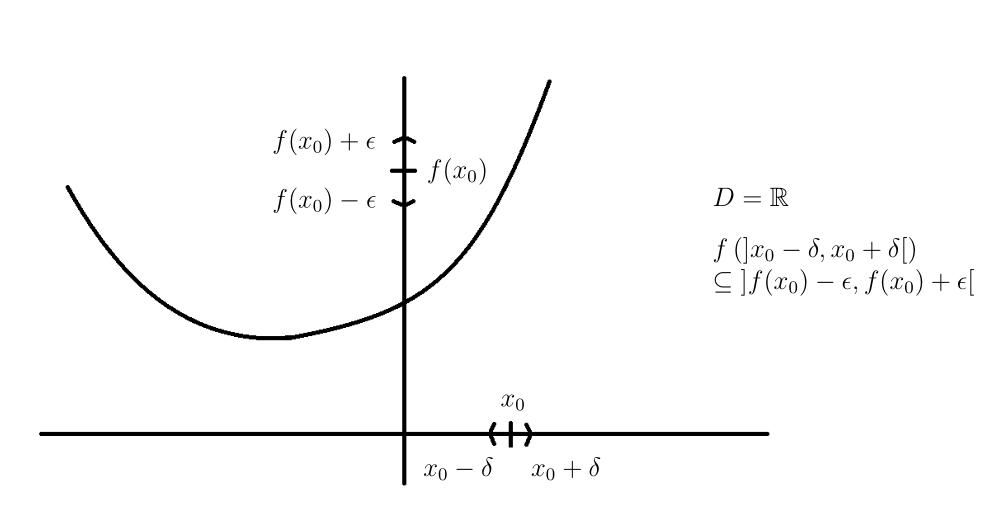
\includegraphics[scale=0.210]{Stetigkeit.png}
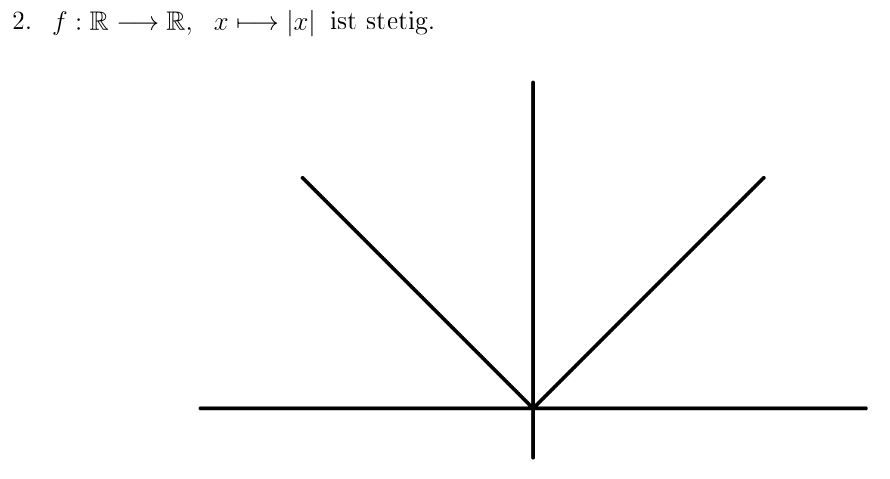
\includegraphics[scale=0.220]{Stetig2.png}
Die Abrundungsfunktion \( \lceil \cdot \rceil : \R \rightarrow \R, x \rightarrow \lceil x \rceil := \max \{ m \in \Z: m \leq z\}\)
ist in jedem Punkt \( x_0 \notin \Z \) stetig; sie ist in keinem Punkt \(y \in \Z \) stetig.
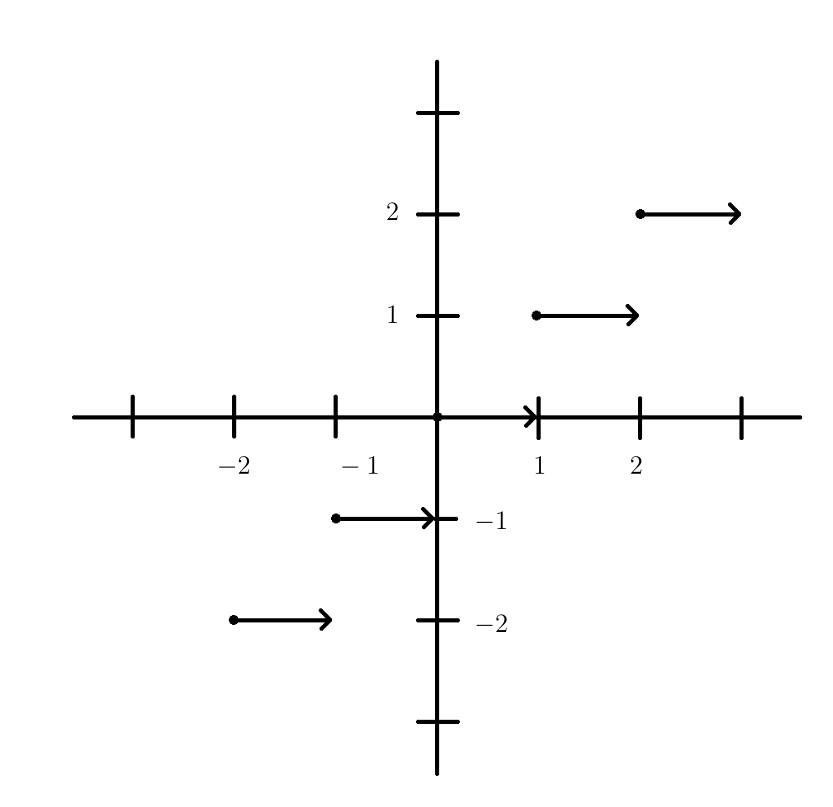
\includegraphics[scale=0.200]{Stetigkeit3.png}
Die Funktion \(f : \R \rightarrow \R \) definiert durch:

\Def[3.5] Die Funktion \(f : D \rightarrow \R\) ist \textbf{stetig}, falls sie in jedem Punkt von D stetig ist. \newline
\Satz[3.7] Sei \(x_0 \in D \subseteq \R \) und \(f: D \rightarrow \R \). Die Funktion f ist genau dann in \(x_0\) stetig falls für jede Folge \((a_n)_{n \geq 1}\) in D folgende implikation gilt:
\[\lim\limits_{n \rightarrow \infty} a_n = x_0 \implies \lim\limits_{n \rightarrow \infty} f(a_n) = f(x_0)\]
\Korollar[3.8] Sei \(x_0 \in D \subseteq \R, \lambda \in \R \) und \(f : D \rightarrow \R, \) \newline \( g: D \rightarrow \R\) beide stetig in \(x_0\)
\begin{enumerate}
    \item [1] Dann sind \(f+g, \lambda \cdot f, f \cdot g\) stetig in \(x_0\)
    \item [2] Falls \(g(x_0) \neq 0\) dann ist
    \[ \frac{f}{g} : D \cap \{x \in D : g(x) \neq 0\} \rightarrow \R\]
    \[x \rightarrow \frac{f(x)}{g(x)}\] stetig in \(x_0\)
\end{enumerate}
\Def[3.9] Eine \textbf{polynomiale Funktion} \(P: \R \rightarrow \R\) ist eine Funktion der Form
\[P(x) = a_nx^n + \dots + a_0\]
wobei : \(a_n \dots a_0 \in \R\). Falls \(a_n \neq 0\) ist n der \textbf{Grad} von P \newline
\Korollar[3.10] Polynomiale Funktionen sind auf ganz \(\R\) stetig \newline
\Korollar[3.11] Seien P,Q, polynomiale Funktionen auf \(\R\) mit \(Q \neq 0\). Seien \(x_1 \dots x_m\) die Nullstellen von Q. Dann ist
\[\frac{P}{Q} : \R \setminus \{x_1, \dots x_m\} \rightarrow \R \]
\[x \rightarrow \frac{P(x)}{Q(x)}\] stetig
\sep
\subsection{Der Zwischenwertsatz}
\Satz[3.12] (Bolzano 1817). Sei \(I \subseteq \R \) ein Intervall, \(f : I \rightarrow \R \) eine stetige Funktion und \(a,b \in I\). Für jedes \(c\) zwischen \(f(a)\) und \(f(b)\) gibt es ein \(z\) zwischen a und b mit \(f(z) = c\) \newline
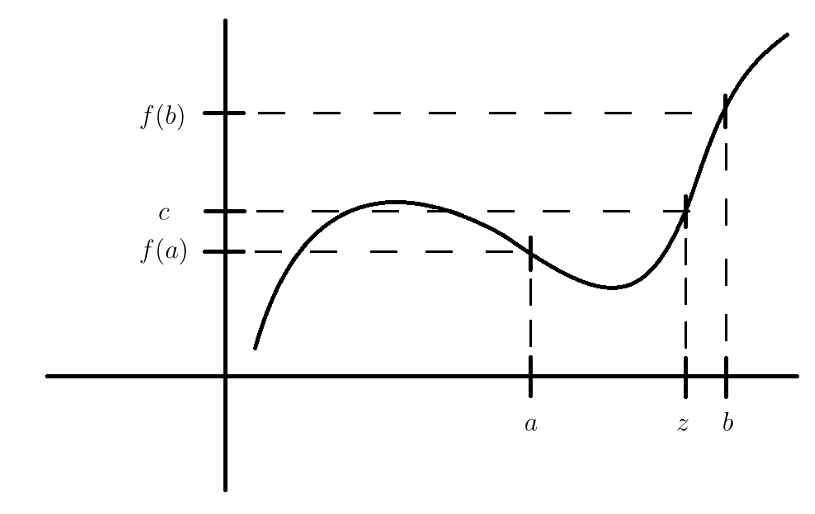
\includegraphics[scale=0.200]{Zwischenwertsatz.png}
\Korollar[3.13] Sei \(P(x) = a_nx^n + a_{n-1}x^{n-1} + \dots + a_0\) ein Polynom mit \(a_n \neq 0\) und \(n\) ungerade. Dann besitzt P mindestens eine Nullstelle in \(\R\) \newline
\Bem[3.14] für \(c > 0\) besitzt \(Q(x) = x^2 + c\) keine Nullstelle in \(R\) \newline
\sep
\subsection{Der Min-Max Satz}
\Def[3.16] Ein Intervall \(\subseteq \R\) ist \textbf{kompakt}, falls es von Form
\[I = [a.b], \quad a \leq b\] ist \newline
\Lemma[3.17] Sei \(D \subseteq \R, x_0 \in D \) und \(f,g : D \rightarrow \R \) stetig in \(x_0\). Dann sind
\[ \abs{f}, \max(f,g), \min(f,g) \] stetig in \(x_0\) \newline
\Lemma[3.18] Sei \((x_n)_{n \geq 1}\) eine konvergente Folge in \(\R\) mit Grenzwert
\[\lim\limits_{n \rightarrow \infty} x_n \in \R \]
sei \(a \leq b\). Falls \(\{x_n : n \geq 1\} \subseteq [a,b]\) folgt
\[\lim\limits_{n \rightarrow \infty} x_n \in [a,b] \]
\Satz[3.19] Sei \(f : I = [a,b] \rightarrow \R \) stetig auf dem kompakten Intervall I. Dann gibt es \(u \in I \) und \(v \in I\) mit
\[f(u) \leq f(x) \leq f(v) \quad \forall x \in I\]
Insbesondere ist f beschränkt
\sep
\subsection{Der Satz über  Umkehrabbildung} 
\Satz[3.20] Seien \(D_1, D_2 \subseteq \R \ zwei \ Teilmengen,\) \newline \(f: D_1 \rightarrow D_2, g: D_2 \rightarrow \R\) Funktionen, sowie \(x_0 \in D_1\). Falls \(f\) in \(x_0\) und \(g\) in \(f(x_0)\) stetig sind
\[ g \circ f : D_1 \rightarrow \R \]
in \(x_0\) stetig \newline
\Korollar[3.21] Falls in Satz 3.20 \(f\) auf \(D_1\) und \(g\) auf \(D_2\) stetig sind, so ist \(g \circ f\) auf \(D_1\) stetig \newline
\Satz[3.22] Sei \(I \subseteq \R\) ein Intervall und \(f: I \rightarrow \R\) stetig, streng monoton. Dann ist \(J:= f(I) \subseteq \R\) ein Intervall und \(f^{-1} : J \rightarrow I \) ist stetig. streng monoton.
\sep
\subsection{Die reelle Exponentialfunktion}
\Def[Exponentialfunktion] \[ \exp(z) := \sum_{n=0}^{\infty} \frac{z^n}{n!}\]
\Satz[3.24] \(\exp: \R \rightarrow ]0,+\infty[\) ist streng monoton wachsend, stetig und surjektiv \newline
\Korollar[3.25] \[ \exp(x) > 0 \quad \forall x \in \R \]
\[\exp(x) > 1 \quad \forall x > 0\] \newline
\Korollar[3.26] \[\exp(z) > \exp(y) \quad \forall z > y\]
\Korollar[3.27] \[\exp(x) \geq 1 + x \quad \forall x \in \R\]
\Korollar[3.28] Der natürliche Logarithmus
\[\ln : ]0,+\infty[ \longrightarrow \R \] ist eine streng monoton wachsende, stetige, bijektive Funktion. Des Weiteren gilt:
\[\ln(a \cdot b) = \ln a + \ln b \quad \forall a,b \in ]0,+\infty[\]
Wir können den Logarithmus und die Exponentialfunktion benutzen, um allgemeine Potenzen zu definieren. Für \(x > 0\) und \( a \in \R \) beliebig definieren wir:
\[ x^a := \exp( a \ln x)\]
Insbesondere \( x^0 = 1 \quad \forall x > 0\) \newline
\Korollar[3.29]
\begin{enumerate}
    \item [1] Für \(a > 0\) ist \[]0,+\infty[ \longrightarrow ]0,+\infty[\]
    \[x \longrightarrow x^a\] eine stetige, streng monoton wachsende Bijektion \newline
    \item [2] Für \(a < 0\) ist \[]0,+\infty[ \longrightarrow ]0,+\infty[\]
    \[x \longrightarrow x^a\] eine stetige, streng monoton fallende Bijektion
    \item [3] \(ln(x^a) = a \ln(x) \quad \forall a \in \R, \forall x > 0\)
    \item [4] \(x^a \cdot x^b = x^{a+b} \quad \forall a,b \in \R, \forall x > 0\)
    \item [5] \((x^a)^b = x^{a \cdot b} \quad \forall a,b \in \R, \forall x > 0\)
\end{enumerate}
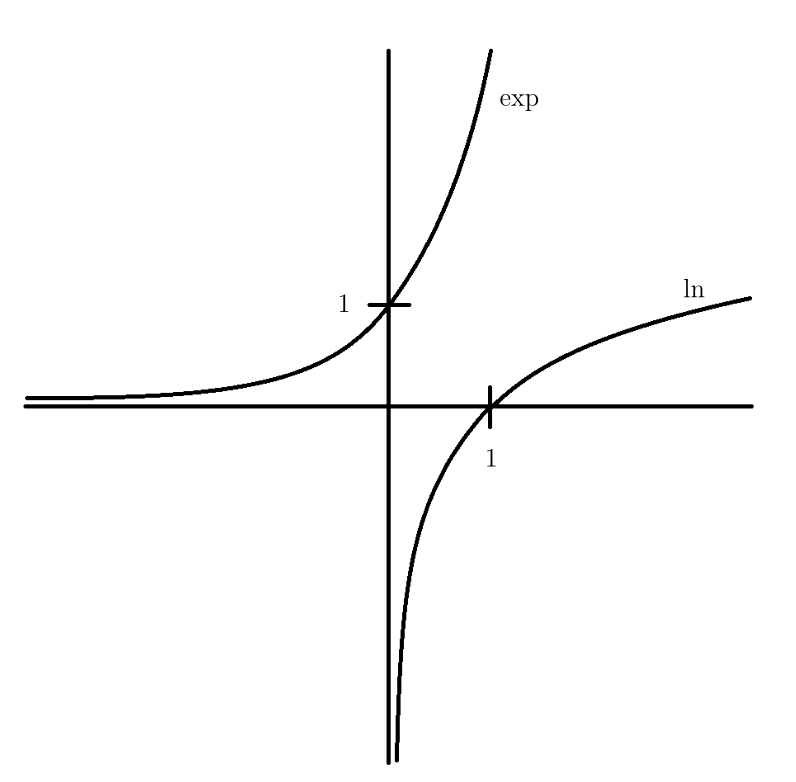
\includegraphics[scale=0.255]{lnExp.png}
\sep
\subsection{Konvergenz v. Funktionenfolgen}
Eine Funktionenfolge ist eine Abbildung 
\[ \N \longrightarrow \R^D\]
\[ n \longrightarrow f(n)\]
\Def[3.30] Die Funktionenfolge \((f_n)_{n \geq 0}\) \textbf{konvergiert punktweise} gegen eine Funktion \(f: D \rightarrow \R\), falls für alle \(x \in D :\)
\[f(x) = \lim\limits_{n \rightarrow \infty}f_n(x)\]
\Def[3.32] (Weierstrass 1841) Die Folge
\[f_n : D \longrightarrow \R \]
\textbf{konvergiert gleichmässig} in D gegen
\[f : D  \rightarrow \R\]
falls gilt \( \forall \epsilon > 0 \quad \exists N \geq 1\), so dass
\[\forall n \geq N,\  \forall x \in D :\  \abs{f_n(x) - f(x) } < \epsilon \] \newline
In dieser Definition ist es wichtig, dass \(N\) nur von \( \epsilon\) abhängig ist und nicht von \(x \in D\).Deswegen kommt die Bedingung \(\forall x \in D\) nach der Bedingung \(\exists N \geq 1\)
\Satz[3.33] Sei \(D \subseteq \R\) und \(f_n : D \rightarrow \R \) eine Funktionenfolge bestehend aus(in D) stetigen Funktionen die (in D) gleichmässig gegen eine Funktion \(f: D \rightarrow \R \) konvergiert. Dann ist \(f\) (in D) stetig \newline
\Def[3.34] Eine Funktionenfolge
\[f_n : D \longrightarrow \R\]
ist \textbf{gleichmässig konvergent}, falls für alle \(x \in D\) der Grenzwert
\[f(x) := \lim\limits_{n \rightarrow \infty} f_n(x)\]
existiert und die Folge \((f_n)_{n \geq 0}\) gleichmässig gegen \(f\) konvergiert \newline
\Korollar[3.35] Die Funktionenfolge
\[f_n : D \longrightarrow \R \]
konvergiert genau dann gleichmässig in D, falls
\[\forall \epsilon > 0 \quad \exists N \geq 1 , \text{so dass} \  \forall n,m \geq N \ \text{und} \ \forall x \in D:\]  \newline
\[ \abs{f_n(x) - f_m(x)} < \epsilon \]
\Korollar[3.36] Sei \(D \subseteq \R\). Falls \(f_n : D \longrightarrow \R \) eine gleichmässig konvergente Folge stetiger Funktionen ist, dann ist die Funktion
\[f(x) := \lim\limits_{n \rightarrow \infty} f_n(x)\] stetig \newline
\Def[3.37] \(f_n: D \longrightarrow \R\) eine Folge von Funktionen. Die Reihe \(\sum_{k=0}^\infty f_k(x)\) konvergiert gleichmässig (in D), falls die durch
\[S_n(x) := \sum_{k=0}^{n}f_k(x)\] definierte Funktionenfolge gleichmässig konvergiert
\Satz[3.38] Sei \(D \subseteq \R \) und
\[f_n : D \rightarrow \R \]
eine Folge stetiger Funktionen. Wir nehmen an
\[\abs{f_n(x)} < c_n \quad \forall x \in D \]
und, dass \(\sum_{n=0}^\infty c_n\) konvergiert. Dann konvergiert die Reihe
\[\sum_{n=0}^\infty\ f_n(x)\]
gleichmässin in D und deren Grenzwert
\[f(x) := \sum_{n=0}^{\infty} f_n(x)\]
ist eine in D stetige Funktion \newline
\Def[3.39] Die Potenzreihe
\[\sum_{k=0}^\infty c_kx^k\]
hat \textbf{positiven Konvergenzradius}, falls \(\limsup\limits_{k \rightarrow \infty} \sqrt[k]{\abs{c_k}}\) existiert
Der Konvergenzradius ist dann definiert als:
\[\rho = \begin{cases}
    +\infty \quad \quad \quad \quad \quad \  \text{falls} \limsup_{k \rightarrow \infty} \sqrt[k]{\abs{c_k}} = 0 \\
    \frac{1}{\limsup\limits_{c \rightarrow \infty} \sqrt[k]{\left|c_{k}\right|}}  \quad \  \ \text{falls } \limsup_{k \rightarrow \infty} \sqrt[k]{\abs{c_k}} > 0
    \end{cases}\]
\newline
\Satz[3.40] Sei \(\sum_{k=0}^\infty c_kx^k \) eine Potenzreihe mit positivem Konvergenzradius \(\rho > 0\) und sei 
\[f(x) := \sum_{k=0}^\infty c_kx^k, \abs{x} < \rho \]
Dann gilt: \(\forall 0 \leq r < \rho \) konvergiert
\[\sum_{k=0}^\infty c_kx^k \]
gleichmässig auf \([-r,r]\), insbesondere ist \newline \(f: ] -\rho,\rho [ \longrightarrow \R\) stetig \newline
\sep
\subsection{Trigonometrische Funktionen}
\Def[Sinus\&Cosinus] \[ \sin(z) = z - \frac{z^3}{2!}+\frac{z^5}{5!}-\frac{z^7}{7!}+ \dots = \sum_{n=0}^{\infty} \frac{(-1)^nz^{2n+1}}{(2n)!}\]
\[ \cos(z) = 1-\frac{z^2}{2!}+\frac{z^4}{4!}-\frac{z^6}{6!}+\dots = \sum_{n=0}^{\infty} \frac{(-1)^nz^{2n}}{(2n)!}\]
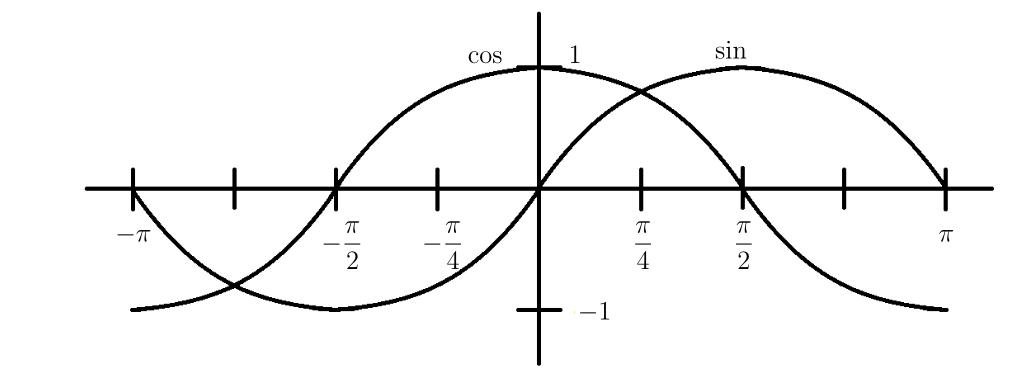
\includegraphics[scale=0.200]{SinCos.png}
\Satz[3.41] \( \sin: \R \rightarrow \R \) und \(\cos: \R \rightarrow \R \) sind stetige Funktionen \newline
\Satz[3.42]
\begin{enumerate}
    \item [1] \( \exp iz = \cos(z) + i \ sin(z) \quad \forall z \in \C \)
    \item [2] \( \cos(z) = \cos(-z)\) und \newline \(\sin(-z) = -\sin z \quad \forall z \in \C \)
    \item [3] \( \sin z = \frac{e^{iz} - e^{-iz}}{2i}, \cos z = \frac{e^{iz} - e^{-iz}}{2}\)
    \item [4] \( \sin(z + w) = \sin(z) \cos(w) + \cos(z) \sin(w)\) \newline
    \( \cos(z + w) = \cos(z) \cos(w) - \sin(z) \sin(w) \)
    \item [5] \( \cos(z)^2 + \sin(z)^2 = 1 \quad \forall z \in \C \)
\end{enumerate}
\Korollar[3.34]
\[\sin(2z) = 2 \sin(z) \cos(z)\]
\[\cos(2z) = \cos(z)^2 - \sin(z)^2\]
\sep
\subsection{Die Kreiszahl \( \pi \)}
\Satz[3.44] Die Sinusfuktion hat auf \(]0,+ \infty [\) mindestens eine Nullstelle
\[ \pi := \inf\{t > 0 : \sin t = 0\}\]
Dann gilt:
\begin{enumerate}
    \item [1] \( \sin \pi = 0,\quad \pi \in ]2,4[\)
    \item [2] \( \forall x \in ]0,\pi [: \sin x > 0\)
    \item [3] \( e^\frac{i \pi}{2} = i\)
\end{enumerate}
\Korollar[3.45]
\[ x \geq \sin x \geq x - \frac{x^3}{3!} \quad \forall 0 \leq x \leq \sqrt{6}\]
\Korollar[3.46]
\begin{enumerate}
    \item [1] \(e^{i \pi} = -1, \quad e^{2 i \pi} = 1\)
    \item [2] \( \sin(x + \frac{\pi}{2}) = \cos(x), \) \newline \(\cos(x + \frac{\pi}{2}) = -  \sin(x) \quad \forall x \in \R\)
    \item [3] \( \sin(x + \pi ) = - \sin(x), \) \newline \( \sin(x + 2 \pi) =  \sin(x) \quad \forall x \in \R \)
    \item [4] \( \cos (x + \pi) = - \cos(x), \) \newline \(\cos(x + 2 \pi) = \cos(x) \quad \forall x \in \R \)
    \item [5] Nullstellen von Sinus = \(\{ k \cdot \pi : k \in \Z\}\)
    \[ \sin(x) > 0 \quad \forall x \in ]2k \pi, (2k + 1) \pi [ ,\quad k \in \Z\]
    \[ \sin(x) < 0 \quad \forall x \in ](2k+1) \pi, (2k + 2) \pi [, \quad k \in \Z\]
    \item [6] Nullstellen von Cosinus \(= \{ \frac{\pi}{2} + k \cdot \pi : k \in \Z \}\)
    \( cos(x) > 0 \) \newline \(\quad \forall x \in ] -\frac{\pi}{2} + 2k \pi, -\frac{\pi}{2} + (2k+1) \pi [, \quad k \in \Z\)
    \( cos(x) < 0 \) \newline \(\forall x \in ] -\frac{\pi}{2} + (2k+1) \pi, -\frac{\pi}{2} + (2k + 2) \pi[,\quad k \in \Z\)
\end{enumerate}
Für \(z \notin \frac{\pi}{2} + \pi \cdot \Z \) definieren wir:
\[\tan(z) = \frac{\sin(z)}{\tan(z)}\]
und für \( z \notin \pi \cdot \Z\) :
\[\cot(z) = \frac{\cos(z)}{\sin(z)}\]
\sep
\subsection{Grenzwerte von Funktionen}
\Def[3.47] \(x_0 \in \R \) ist ein \textbf{Häufungspunkt} der Menge D falls \( \forall \delta > 0\) : 
\[ (]x_0 - \delta, x_0 + \delta [ \setminus \{x_0\}) \cap D \neq \emptyset \]
\Def[3.49] Sei \( f: D \longrightarrow \R, x_0 \in \R \) ein Häufungspunkt von D. Dann ist \(A \in \R \) der Grenzwert von \(f(x)\) für \(x \rightarrow x_0\) bezeichnet mit
\["\lim\limits_{x \rightarrow x_0} f(x) = A"\]
falls \( \forall \epsilon > 0 \quad \exists \delta > 0\) so dass
\[ \forall x \in D \cap (] x_0 - \delta, x_0 + \delta [ \setminus \{x_0\}) : \abs{f(x) - A } < \epsilon\]
\Bem{3.50}
\begin{enumerate}
    \item [1] Sei \(f : D \rightarrow \R \) und \(x_0\) ein Häufungspunkt von D. Dann gilt \(\lim\limits_{x \rightarrow x_0} f(x) = A \) genau dann wenn für alle Folgen \((a_n)_{n \geq 1 }\) in \(D \setminus \{x_0\}\) mit
    \[ \lim\limits_{n \rightarrow \infty} a_n = x_0  \]
    folgt
    \[ \lim\limits_{n \rightarrow \infty} f(a_n) = A \]
    \item [2] Sei \(x_0 \in D. \) Dann ist f stetig in \(x_0\) genau dann, falls
    \[ \lim\limits_{x \rightarrow x_0} f(x) = f(x_0)\]
    \item [3] Falls \(f,g : D \rightarrow \R \) und \( \lim\limits_{x \rightarrow x_0} f(x), \lim\limits_{x \rightarrow x_0} g(x)\) existieren, so folgt
    \[\lim\limits_{x \rightarrow x_0}(f + g)(x) = \lim\limits_{x \rightarrow x_0} f(x) + \lim\limits_{x \rightarrow x_0} g(x)\]
    und
    \[\lim\limits_{x \rightarrow x_0}(f \cdot g)(x) = \lim\limits_{x \rightarrow x_0} f(x) \cdot \lim\limits_{x \rightarrow x_0} g(x)\]
    \item [4] Sei \(f,g : D \rightarrow \R \) mit \(f \leq g \). Dann folgt
    \[\lim\limits_{x \rightarrow x_0} f(x) \leq \lim\limits_{x \rightarrow x_0} g(x)\]
    falls beide Grenzwerte existieren
    \newline\newline
    \item [5] Falls \(g_1 \leq f \leq g_2\) und
    \[ \lim\limits_{x \rightarrow x_0} g_1(x) = \lim\limits_{x \rightarrow x_0} g_2(x)\]
    dann existiert \(\lim\limits_{x \rightarrow x_0} f(x)\) und
    \[ \lim\limits_{x \rightarrow x_0} f(x) = \lim\limits_{x \rightarrow x_0} g_1(x )\]
\end{enumerate}
\Satz[3.52] Seien \(D,E \subseteq \R,\  x_0 \) Häufungspunkt von \(D, f: D \longrightarrow E \) eine Funktion. Wir nehmen an, dass
\[y_0 := \lim\limits_{x \rightarrow x_0} f(x)\]
existiert und \(y_0 \in E.\) Falls \(g: E \longrightarrow \R \) stetig in \(y_0\) folgt:
\[ \lim\limits_{x \rightarrow x_0} g(f(x)) = g(y_0)\]
\sep
\subsection{Linksseitige und rechsseitige Grenzwerte}
Betrachten wir zum Beispiel
\[f: \R \setminus \{0\} \longrightarrow \R\]
\[x \longrightarrow \frac{1}{x}\]
Dann wird für \( x > 0\), x beliebig nahe an 0, \(\frac{1}{x}\) beliebig positiv gross und für \(x < 0\), x beliebig nahe an 0, \( \frac{1}{x}\) beliebig negativ "gross".In beiden Fällen hat \( \frac{1}{x}\) ein einfaches Verhalten. \newline
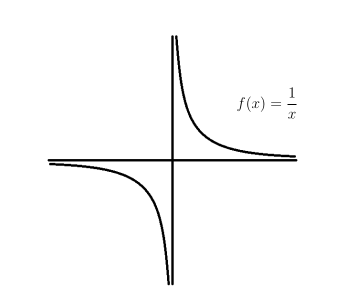
\includegraphics[scale=0.225]{LR-GrenzWert.png} \newline
Im Fall \(a \in \R\),
\[f: ]0,\infty[ \rightarrow \R\]
\[x \rightarrow x^a\]
ist f auf \(]0,\infty[\) definiert. Falls \(a > 0\) werden wir sehen, dass
\[ \lim_{x\in ]0,\infty[\rightarrow 0} f(x) = 0\]
Sei \(f: D \longrightarrow \R \) und \(x_0 \in \R \). Wir nehemn an, \(x_0\) ist Häufungspunkt von \(D \cap ]x_0, +\infty[;\)
das heisst ein rechtsseitiger Häufungspunkt. Falls der Grenzwert der eingeschränkten Funktion
\[f|_{D \cap [x_0,+\infty[}\]
für \(x \longrightarrow x_0\) existiert, wird er mit
\[ \lim_{x \rightarrow x_0^+} f(x)\]
bezeichnet und nennt sicht rechtsseitiger Grenzwert von \(f\) bei \(x_0\).\newline \newline
Wir erweitern diese Definition auf:
\[\lim_{x \rightarrow x_0^+} f(x) = +\infty \]
falls gilt:
\[ \forall \epsilon > 0 \exists \delta > 0, \ \forall x \in D \cap ]x_0,x_0 + \delta[:\ f(x) > \frac{1}{\epsilon}\]
und analog:
\[ \lim_{x \rightarrow x_0^+} f(x) = -\infty \]
falls
\[ \forall \epsilon > 0 \  \exists \delta > 0, \ \forall x \in D \cap ]x_0,x_0+\delta[: f(x) < -\frac{1}{\epsilon}\]
Linksseitige Häufungspunkt und Grenzwerte werden analog definiert. Mit diesen Definitionen gilt:
\[\lim_{x \rightarrow 0^+}\frac{1}{x} = +\infty, \quad\ \lim_{x \rightarrow 0^-}\frac{1}{x} = -\infty \]